\documentclass[12pt]{article}
\usepackage{fontspec}
\usepackage{polyglossia}
\usepackage{wrapfig}
\setdefaultlanguage{russian}
\setmainfont[Mapping=tex-text]{CMU Serif}
\usepackage{minted}
\newfontfamily{\cyrillicfonttt}[Scale=0.8]{Liberation Mono}
%\setdefaultlanguage{russian}
%\setmainfont[Mapping=tex-text]{CMU Serif}

\title{CEL MeshWorks}
\author{Владимир Петриго}
\date{Ноябрь 2015}

\begin{document}

\maketitle

\section{Введение}

Стремительное развитие приобретает концепция Internet of Things (Интернет Вещей),
основной идеи которой является объединение бытовых и не только приборов или 
устройств в единую сеть. И производители очень часто предлагают различные 
средства для ускорения разработки либо для быстрой интеграции в уже существующие 
проекты, где необходимо добавить беспроводную связь или же убрать лишние провода.

Компания CEL выпустила платформу MeshWorks, позволяющую настроить и организовать 
беспроводную ZigBee-сеть не имея особых знаний в программировании встраиваемых систем
либо беспроводного стандарта связи ZigBee. Если стоит задача в короткий срок развернуть
систему сбора данных с аналоговых датчиков или устройств с I2C-интерфейсом либо 
систему управления, используя цифровые входы/выходы, то платформа MeshWorks позволит
это сделать быстро и не вдаваясь в детальные подробности работы с микроконтроллером, 
периферией и обработкой сетевых событий.

Для разработчиков доступны как готовые ZigBee-Ethernet- и ZigBee-USB-шлюзы, 
сенсорные узлы, так и отдельные модули, которые имеют встроенную 
прошивку-интерпретатор. Эта прошивка предоставляет возможность обработки скриптов, 
написанных на специальном скриптовом языке, похожем на язык Python, прямо на 
встроенном микроконтроллере. 
\section{Аппаратная платформа MeshWorks}
Компания CEL в своей линейке продукции, которая поддерживает работу с платформой 
MeshWorks, имеет как модули, так и готовые изделия.
% Module ZICM3588SP2 image
\begin{wrapfigure}{l}{0.3\textwidth}
  \begin{center}
    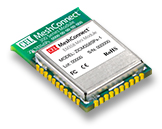
\includegraphics[width=0.25\textwidth]{mc_em358x_mini.jpg}
  \end{center}
  \caption{ZICM3588SP2}
\end{wrapfigure}
Модули ZICM3588SPx и ZICM357SPx построены на базе микросхем EM3588 и EM357 компании
Silicon Labs. Это системы на кристалле с микроконтроллерным ядром ARM Cortex-M3 и
встроенным ZigBee-приемопередатчиком, работающем на частоте 2.4 ГГц. Модули имеют
два исполнения - со встроенным усилителем мощности (максимальная выходная мощность
+20 дБм) и без него (максимальная выходная мощность +8 дБм). Благодаря высокой 
чувствительности встроенного приемопередатчика бюджет радиосвязи может достигать 
+123 дБ, что позволяет достичь дальности радиосвязи на открытых пространствах до 1 км,
а внутри помещений уверенно пробивать через бетонную стену. В таблице 1 представлены
основные характеристики модулей ZICM3588SPx и ZICM357SPx.

\begin{table}[h!]
    \begin{center}
    \caption{Характеристики модулей ZICM3588SPx и ZICM357SPx} 
    \begin{tabular}{|r|c|c|}
    \hline
    {} & \textbf{ZICM3588SPx} & \textbf{ZICM357SPx} \\
    \hline
    SoC & EM3588 & EM357 \\
    \hline
    GPIO & 23 & 19 \\
    \hline
    RAM & 64 Кб & 12 Кб \\
    \hline
    Flash & 512 Кб & 192 Кб \\
    \hline
    Мощность передатчика & \multicolumn{2}{c|}{+8/+20 дБм}\\
    \hline
    Чувствительность & \multicolumn{2}{c|}{-100/-103 дБм}\\
    \hline
    АЦП & \multicolumn{2}{c|}{5-канальный 14-разрядный}\\
    \hline
    Интерфейсы & \multicolumn{2}{c|}{SPI/I2C/UART}\\
    \hline
    USB & + & -\\
    \hline
    Температурный диапазон & \multicolumn{2}{c|}{-40..+85°С (-40..+125°С)}\\
    \hline
    \end{tabular}
    \end{center}
\end{table}
\newpage
Для возможности интегрировать ZigBee-сети с существующими серверными, настольными,
мобильными и прочими приложениями, компания CEL предлагает готовые ZigBee-USB- и 
ZigBee-Ethernet-шлюзы.

% USB and Ethernet Gateway images
\begin{wrapfigure}{l}{0.25\textwidth}
  \begin{center}
    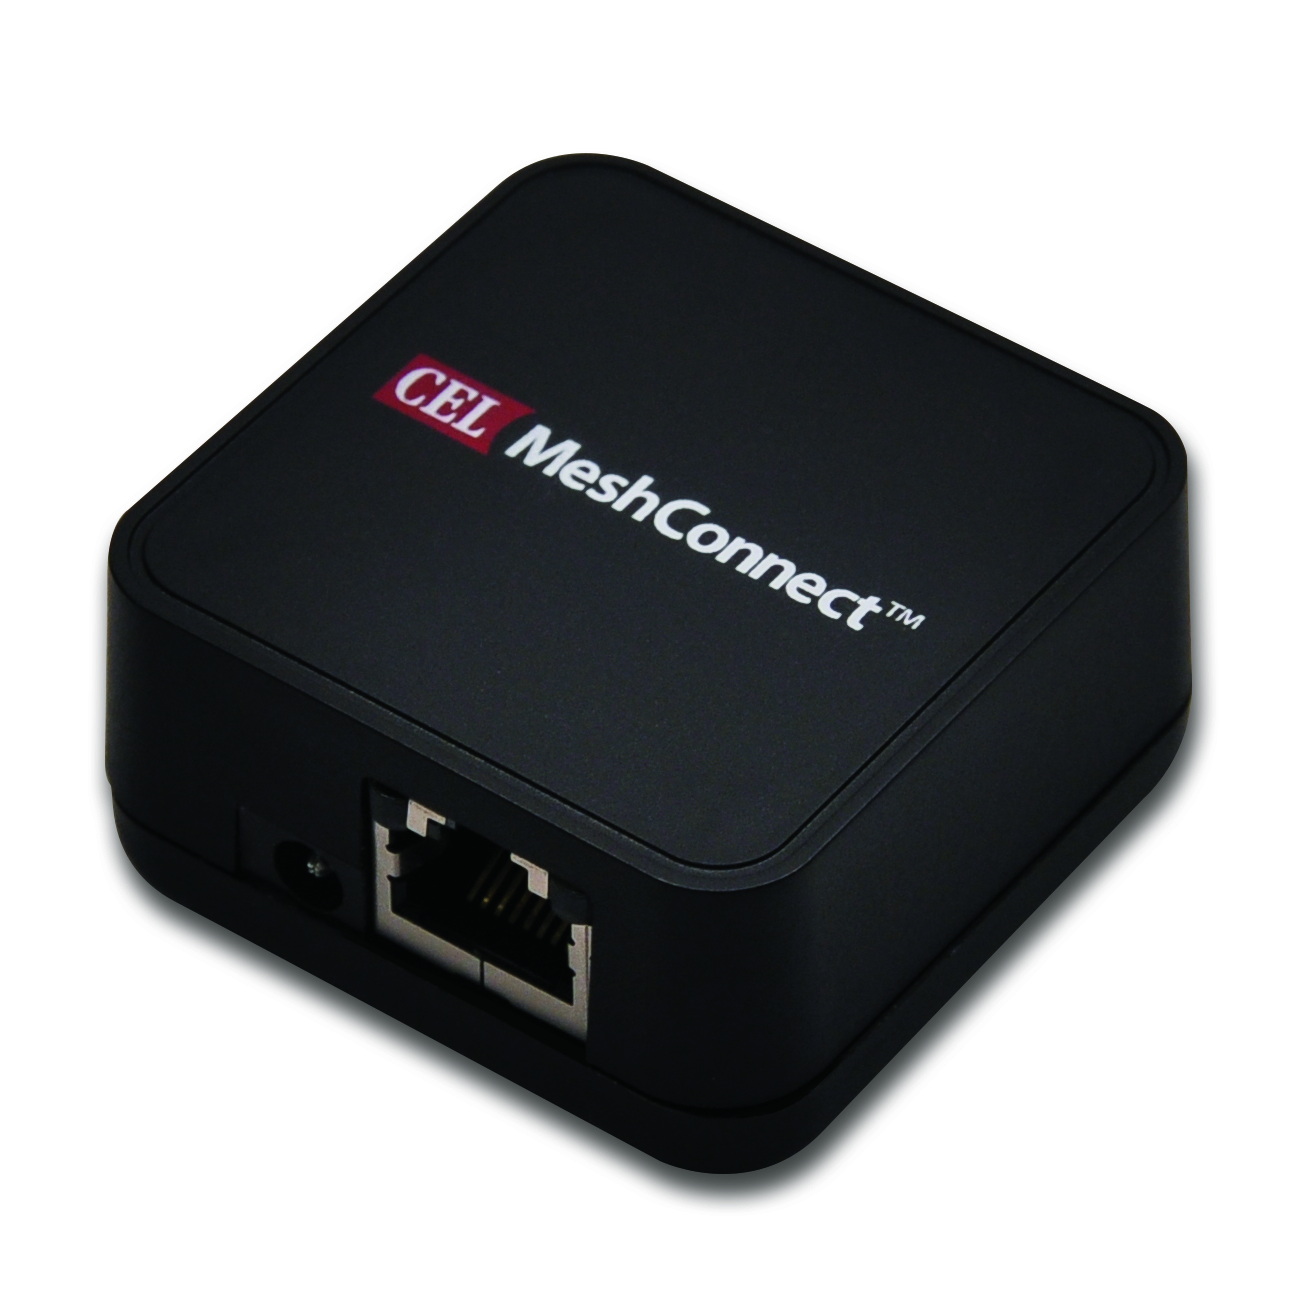
\includegraphics[width=0.20\textwidth]{gateway2.jpg}
  \end{center}
  \caption{ZMC-GW-ETH-1}
  \begin{center}
    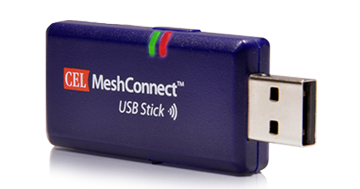
\includegraphics[width=0.20\textwidth]{usb_stick_em358_img_tech_plain.png}
  \end{center}
  \caption{ZM3588S-USB}
\end{wrapfigure}

ZigBee-Ethernet-шлюзы являются полноценными участниками ZigBee-сети и позволяют 
отправлять TCP/UDP/HTTP-сообщения на указанный в приложении адрес и порт. Также
имеется возможность

ZigBee-USB-шлюзы при подключении к компьютеру или другому устройству, распознается
как виртуальный COM-порт. Это позволяет добавить к существующим устройствам 
(например Wi-Fi-роутер с USB-разъемом, в которые можно загрузить собственное приложение;
персональный компьютер и т.д.) добавить возможность работы с сетями ZigBee. Шлюзы
как и модули имеют встроенную прошивку-интерпретатор, которая позволяет загружать
в них скрипты на языке MeshWorks. Шлюзы как и модули построены на базе микросхем
EM357/EM3588, поэтому все характеристики, справедливые для модулей и приведенные
в таблице 1, справедливы и для них.
\\\\
Кроме модулей и шлюзов для оценки возможности платформы MeshWorks предлагаются 
готовые сенсорные узлы OpenTether, имеющие в своем составе ряд датчиков и набор периферии:
\begin{itemize}
    \item датчик влажности и температуры Si7013 (с интерфейсом I2C)
    \item акселерометр, гироскоп и компас MPU-9250 (с интерфейсом I2C)
    \item датчик близости Si1143-M01 (с интерфейсом I2C)
    \item геркон
    \item 2 светодиода
    \item кнопка
    \item сирена
    \item разъем для подключения внешних устройств (аналоговых датчиков, I2C-устройств,
    цифровых входов/выходов)
\end{itemize}

% OpenTether image
\begin{wrapfigure}{l}{0.28\textwidth}
  \begin{center}
    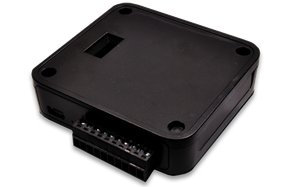
\includegraphics[width=0.20\textwidth]{sensor_node.png}
  \end{center}
  \caption{OpenTether}
\end{wrapfigure}

Данный сенсорный узел дает возможность простого прототипирования и отладки приложения.
Имеется несколько возможностей для питания сенсорного узла:
\begin{itemize}
 \item micro-USB-разъем
 \item 2xAAA батарейки
 \item DC-разъем (2.1 - 3.6 В)
\end{itemize}

По USB-интерфейсу осуществляется загрузка скрипта в подключенное устройство, либо 
его отправка на удаленный узел. Также по USB-интерфейсу осуществляется работа с
командным интерфейсом прошивки-интерпретатора, получение пользовательской и служебной
информации.

\section{Пример работы}
В качестве демонстрационного примера решим следующую задачу. Имеется две комнаты,
температуру в которых необходимо измерить, а также есть два выключателя, которые
должны управлять состоянием лампочек. И все данные о температуре и состоянии
выключателей должны передаваться на централизованный сервер. Примерная структурная
схема представлена на рисунке 1.
\begin{figure}[h!]
    \centering
    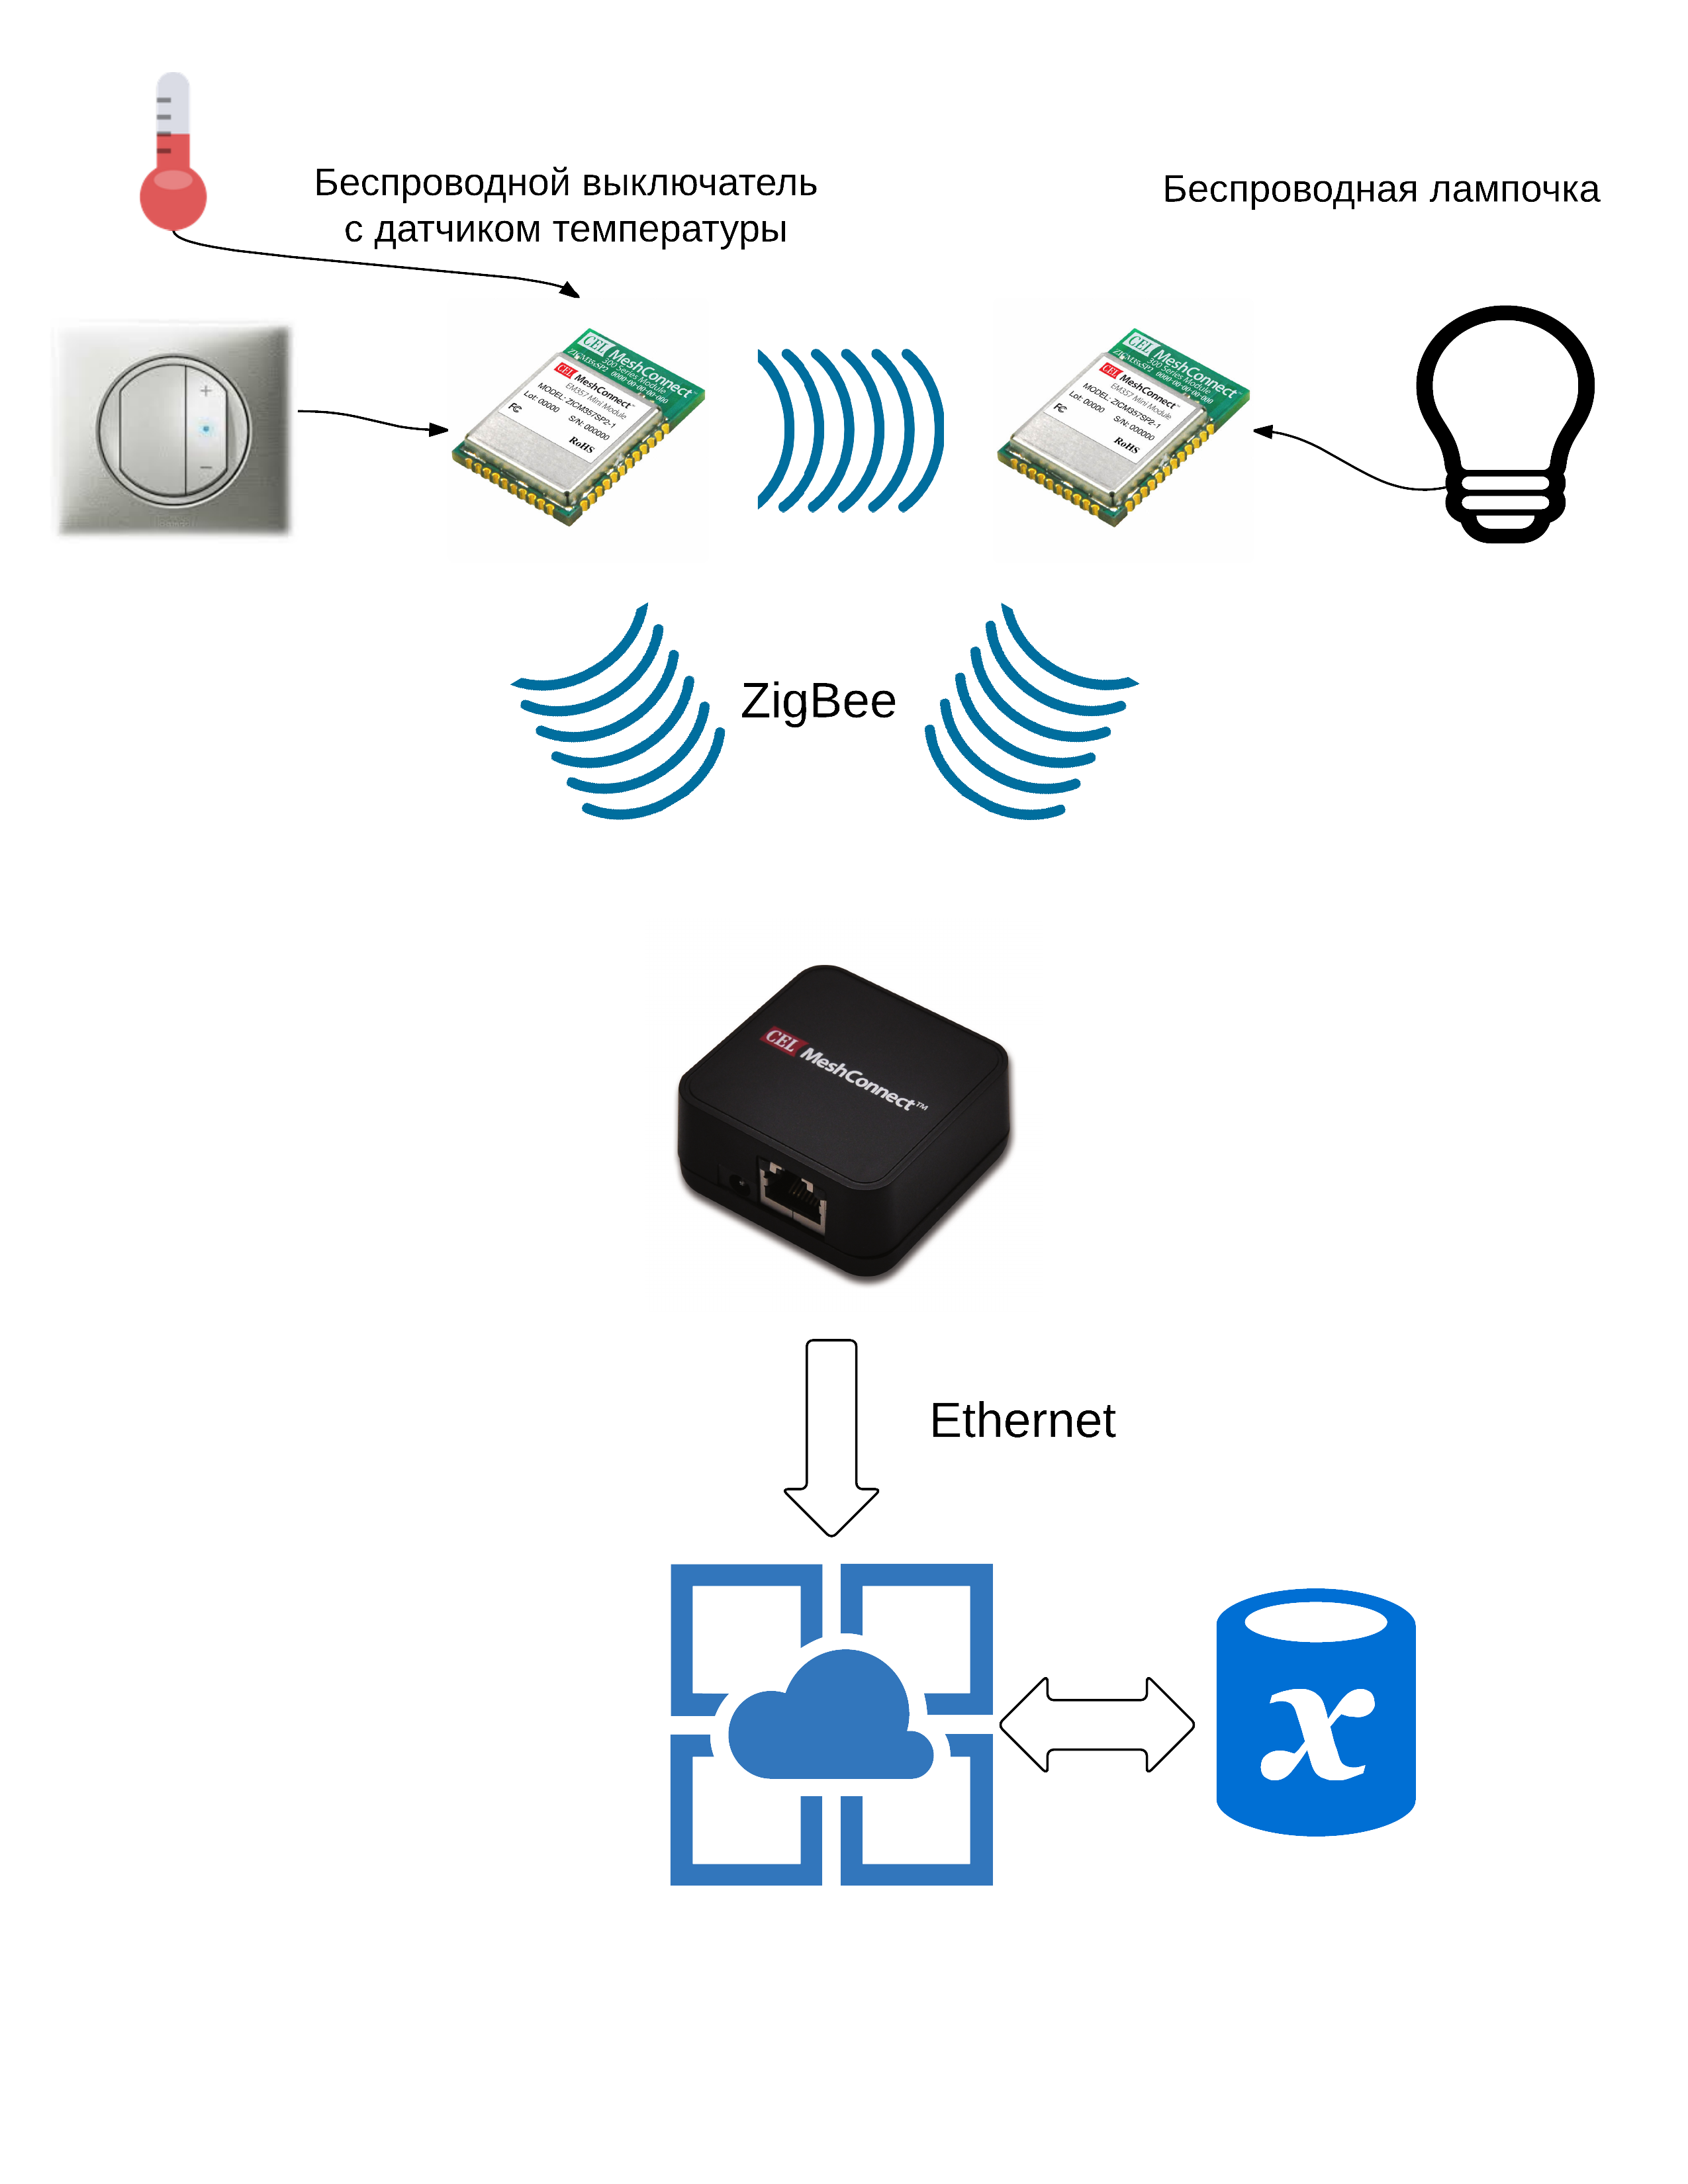
\includegraphics[scale=0.5]{cel-structure.png}
    \caption{Структурная схема примера}
\end{figure}

Выключатель, ламочка подключены к цифровым входам модуля CEL ZICM3588, в качестве
датчика температуры используется однокристальный датчик влажности и температуры
Si7013 с I2C-интерфейсом.

При изменении состояния выключателя лампочка включается или выключается. Также 1 раз в 20
секунд обновляется информация о значении температуры в комнате. Информацию об этом
каждый узел передает по радиоканалу на центральный шлюз. Центральный шлюз всю
полученную информацию передает на локальный или глобальный сервер.

Пример скрипта для узла сбора данных:
\begin{minted}{python}
    # Светодиод на выводе PA6 
    greenLed = ["greenLed", "PA6", "digital", "grLedF", 1]
    greenValues = ["discrete", 2, "off", "on"]
    # Светодиод на выводе PA7 
    redLed = ["redLed", "PA7", "digital", "rdLedF", 1]
    redValues = ["discrete", 2, "off", "on"]
      
    # Data Point для кнопки
    button = ["button", "PB6", "digital", "buttonF", 1] 
    bValues = ["discrete", 2, "up", "down"] 
    
    prevButtonValue = 0
    buttonTickCount = 0 
      
    def buttonF():
        value = readDigital()
        # Периодическая отправка данных
        # о состоянии выключателя
        if (buttonTickCount > 30):
            buttonTickCount = 0
            sendDataReport(value, "button state")
        # если значение поменялось 
        if (value != prevButtonValue):  
            sendDataReport(value, "button state")
            # Устанавливаем состояние светодиода
            # в соответствии с состоянием выключателя
            celPy.AdjustLocalControlPoint("greenLed", value)    
        prevButtonValue = value
        buttonTickCount = (buttonTickCount + 1)
        
    # Data Point для датчика температуры
    tempSensor = ["tempSensor", "PA1", "i2c", "tempMeasFunc", 20]
    tempSensorValues = ["range", -40, 120]
    
    # Чтение температуры с Si7013
    def tempMeasFunc():
        value = readI2c(0x41, 0xE3, bigEndian)
        # Преобразование в градусы Цельсия
        value = (value * 175)
        value = (value / 65535)
        value = (value - 47)
        sendDataReport(value, "degrees C")
    
    celPy.addTickFunction(heartbeatLed, 20) 
      
    ledState = 0
      
    def heartbeatLed(): 
        if (ledState == 0): 
            celPy.AdjustLocalControlPoint("redLed", 1)
            ledState = 1
            return
        if (ledState == 1): 
            celPy.AdjustLocalControlPoint("redLed", 0)
            ledState = 0
      
    ####################################################
    # Сетевые настройки
    celPy.ApplicationName = "MeshWorks"  
    celPy.DeviceName = "Sensor 1" 
    celPy.IsSleepyDevice = False
    celPy.DataCollectionPoints = [button, tempSensor] 
    celPy.DataCollectionValues = [bValues, tempSensorValues]
    celPy.ControlPoints = [greenLed, redLed]
    celPy.ControlValues = [greenValues, redValues] 
      
    def main(): 
        pass
\end{minted}

Функциональность устройства определятся тремя основными функциями:
\begin{itemize}
    \item \emph{buttonF()} -- обрабатывает нажатие на кнопку (выключатель). При 
    изменении состояния светодиод (лампочка) переключается в соответствующее состояние.
    Об этом событии также отправляется сообщение на центральный шлюз. В приведенном
    выше примере также осуществляется отправка информации о текущем состоянии выключателя
    каждые 30 секунд.
    \item \emph{tempMeasFunc()} -- считывает данные с датчика
    Si7013 по интерфейсу I2C, переводит цифровые данные в градусы Цельсия и 
    отправляет эту информацию на центральный шлюз.
    \item \emph{heartbeatLed()} -- индикация работоспособности устройства. Переключает
    состояние вспомогательного красного светодиода каждые 2 секунды.
\end{itemize}

Пример скрипта для центрального Ethernet-шлюза:
\begin{minted}{python}
# Конфигурация шлюза
celPy.ApplicationName = "MeshWorks"
celPy.DeviceName = "Gateway"
celPy.IsSleepyDevice = False

# Обработка сообщений от других сетевых устройств
def cpCallbackDataPointMessageReceived(deviceName, datapointName, discreteValueString, rangeValue):
    if (deviceName == "Sensor 1"):
        if (datapointName == "button"):
            udpPayload = deviceName
            udpPayload = (udpPayload + ": button=")
            udpPayload = (udpPayload + rangeValue)
            udp.send("192.168.22.225", 5555, udpPayload)
        if (datapointName == "tempSensor"): 
            udpPayload = deviceName
            udpPayload = (udpPayload + ": temp=")
            udpPayload = (udpPayload + rangeValue)
            udp.send("192.168.22.225", 5555, udpPayload) 
    if (deviceName == "Sensor 2"):
        if (datapointName == "button"):
            udpPayload = deviceName
            udpPayload = (udpPayload + ": button=")
            udpPayload = (udpPayload + rangeValue)
            udp.send("192.168.22.225", 5555, udpPayload)
        if (datapointName == "tempSensor"): 
            udpPayload = deviceName
            udpPayload = (udpPayload + ": temp=") 
            udpPayload = (udpPayload + rangeValue)
            udp.send("192.168.22.225", 5555, udpPayload)  
   
def main(): 
    pass

\end{minted}

Здесь функциональность определяется одной единственной функцией 
\emph{cpCallbackDataPointMessageReceived}, которая вызывается всякий раз, когда 
на шлюз поступает информация от других сетевых устройств. В зависимости от значения
переменной \emph{datapointName} (имя Data Point отправителя) и \emph{deviceName} (имя 
устройства) формируется соответствующее сообщение и отправляется на указанный адрес
сервера и порт.
\section{Заключение}
Платформа MeshWorks предлагает очень простой интерфейс для быстрой разработки систем
сбора данных, которые позволяют использовать практически все основные функциональные
особенности модулей ZICM3588SP2-1 на базе микросхем EM3588:
\begin{itemize}
 \item Работа с цифровыми портами ввода/вывода
 \item Подключение аналоговых датчиков
 \item Работа с устройствами и датчиками, использующими интерфейс I2C
 \item Поддержка спящих устройств, которые должны работать длительный срок от
 аккумуляторных или батарейных источников питания
\end{itemize}
Кроме этого компания CEL предоставляет устройства с Ethernet- и USB-интерфейсами, 
позволяющими расширить функциональность ZigBee-сетей, на базе платформы MeshWorks.
Это значительно упрощает интеграцию с серверными, настольными и мобильными приложениями.
\end{document}
